% \newcommand\chapternumber{1}
\documentclass[12pt,a4paper]{article}
\usepackage{fullpage}
\usepackage[top=2cm, bottom=4.5cm, left=2.5cm, right=2.5cm]{geometry}
\usepackage{amsmath,amsthm,amsfonts,amssymb,amscd}
\usepackage{lastpage}
\usepackage{enumitem}
\usepackage{fancyhdr}
\usepackage{mathrsfs}
\usepackage{xcolor}
\usepackage{graphicx}
\usepackage{listings}
\usepackage{hyperref}
\usepackage{tikz}
\usetikzlibrary{shapes,backgrounds}
\usepackage[utf8]{inputenc}
\usepackage[ruled, vlined]{algorithm2e}
% \usepackage{apacite}
\usepackage{csquotes}

% Edit these as appropriate
\newcommand\course{Reinforcement Learning}
\newcommand\NetID{sliu1@uvm.edu}
\newcommand\Author{Sida Liu}
\pagestyle{fancyplain}
\headheight 35pt
\lhead{\NetID\\\Author}
% \chead{\textbf{\Large Assignment \chapternumber }}
\rhead{\course \\ \today}
\lfoot{}
\cfoot{}
\rfoot{\small\thepage}
\headsep 1.5em

\setlength{\parskip}{\baselineskip}%
\setlength{\parindent}{0pt}%

\newenvironment{list_abc}
{ \begin{enumerate}[label=(\alph*)] }
{ \end{enumerate} }

\newenvironment{list_iv}
{ \begin{enumerate}[label=\roman*.] }
{ \end{enumerate} }

\hypersetup{
    colorlinks=true,
    linkcolor=blue,
    filecolor=magenta,      
    urlcolor=cyan,
}

\usepackage{tcolorbox}
\usepackage{booktabs}


\begin{document}

\section*{Initial Project Proposal}

\subsection*{Structure}
The deliverable will be a piece of open-source software.

\subsection*{Topic}
In 2017, Yoshua Bengio submitted an arXiv article named \emph{The Consciousness Prior} \cite{bengio_consciousness_2019}. He proposed the \emph{Consciousness Prior Theory}, which his intuition about how the consciousness works and how the \emph{Global Workspace Theory} could be implemented using recently developed \emph{Deep Learning} technology. The article contains a preliminary plan about how all the pieces should come together to create a consciousness that can facilitate the learning process. However, to my best knowledge, there are still no existing experiments that can support his \emph{Consciousness Prior Theory}.

Implementing the whole framework in one semester will be too ambitious. So I am going to implement a minimum embodied toy RL model to showcase part of his theory, more precisely, the abstraction part which produces the high-level abstraction $h$.

In Bengio's paper, he thinks the high-level abstraction $h$ is produced by some representation RNN function $F$, so that

\begin{equation*}
    h_t = F(x_t, h_{t-1})
\end{equation*}

where $x_t$ is the \emph{observation} at time $t$, and $h_{t}$ is the \emph{unconscious representation state} (or \emph{high-level state}) at time $t$.
I think this is very similar to the $RL^2$ paper \cite{duan_rl2_2016}, where $h$ is the hidden states of the RNN. 

If we take the \emph{Hierarchical RL} point of view, $h_t$ can be the \emph{observation} of a high-level RL, and there could be multiple levels of $h$'s. (I am not sure how to automatically define \emph{options} yet, maybe it can be another output of the function $F$.)

Moreover, the recent success of the Transformer model \cite{vaswani_attention_2017} indicates that it is possible to add Attention mechanism to extract $h$ more efficiently. I am going to combine Transformer and RNN if there's enough time.

I plan to use PyTorch to implement the neural networks, and I'll possibly use some other open-source projects (such as stable-baseline3) as sub-modules.

Hope it will work.

HRL diagram:
\begin{figure}[h]
    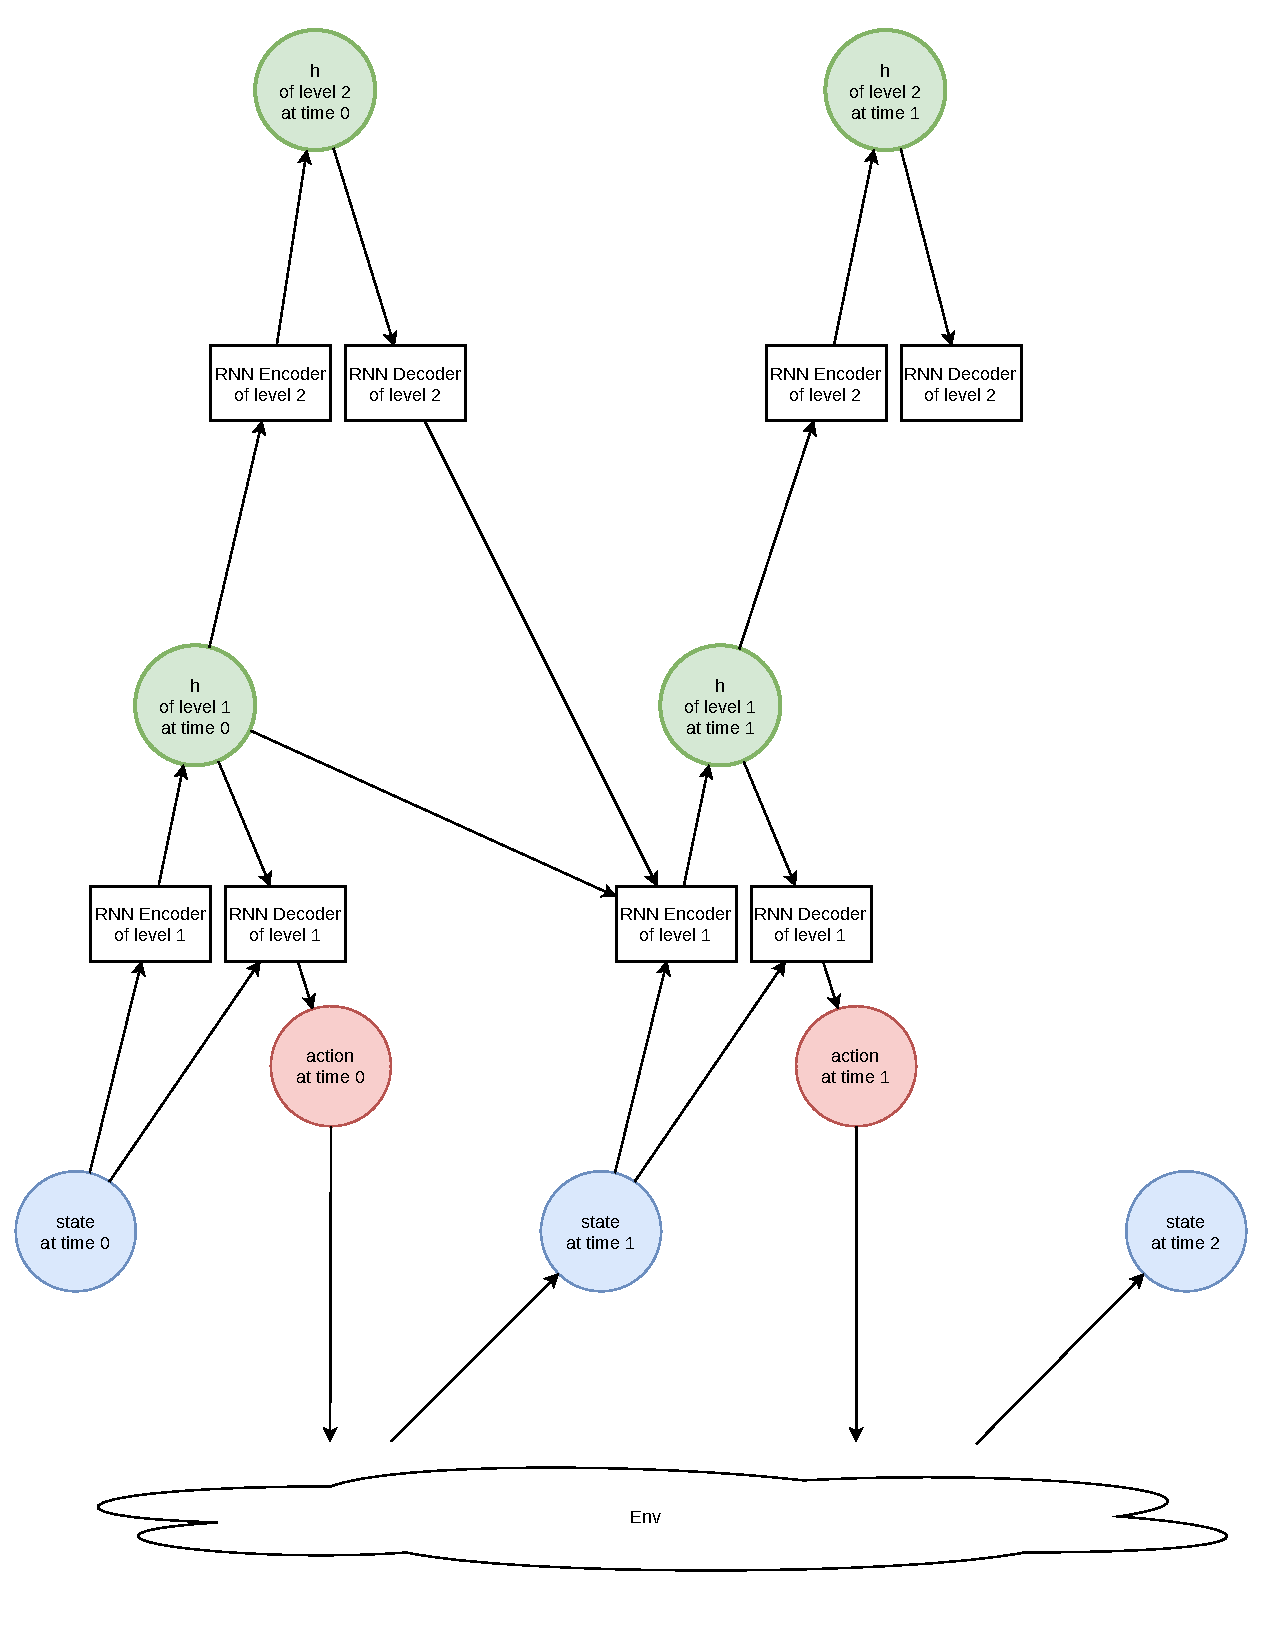
\includegraphics[width=0.8\textwidth]{images/HRL-diagram.pdf}
\end{figure}

\newpage
\bibliographystyle{plain}
\bibliography{reference.bib}


\end{document}
